\documentclass{article}

\usepackage{amsmath}
\usepackage{amssymb}
\usepackage{graphicx}
\usepackage{float} 

\begin{document}

\section*{Problem 1}

Let $S(n,k)$ denote the number of ways to partition
$\{1,2,\ldots,n\}$ into $k$ nonempty, unlabeled subsets.Give a story proof for each of the following identities.


\subsection*{(a)}

prove
\[
S(n+1,k)=S(n,k-1)+kS(n,k).
\]

Consider partitioning the set
\[
\{1,2,\ldots,n,n+1\}
\]
into $k$ nonempty, unlabeled subsets.

\textbf{Case 1:} The element $n+1$ forms a subset by itself.

Then the remaining $n$ elements
\[
\{1,2,\ldots,n\}
\]
must be partitioned into $k-1$ nonempty subsets. There are
\[
S(n,k-1)
\]
ways.

\textbf{Case 2:} The element $n+1$ does not form a subset by itself.

First partition
\[
\{1,2,\ldots,n\}
\]
into $k$ nonempty subsets. This can be done in
\[
S(n,k)
\]
ways.

Then $n+1$ can be placed into any one of these $k$ subsets, giving
\[
kS(n,k)
\]
possibilities.

the two cases are disjoint and cover all possible partitions
\[
\implies
S(n+1,k)=S(n,k-1)+kS(n,k)
\]

\subsection*{(b)}

prove 
\[
S(n,k)=
\sum_{j=k-1}^{n-1}
\binom{n-1}{j}S(j,k-1).
\]

Consider partitioning
\[
\{1,2,\ldots,n\}
\]
into $k$ nonempty, unlabeled subsets.

Focus on the subset containing the element $n$.

Let $j$ denote the number of elements that are not in the same subset as $n$.
These $j$ elements must form the other $k-1$ subsets.

First, choose these $j$ elements from
\[
\{1,2,\ldots,n-1\}.
\]
There are
\[
\binom{n-1}{j}
\]
ways to choose them.
$\because$  partition these $j$ chosen elements into $k-1$ nonempty subsets.
\[
\therefore
S(j,k-1)
\]
ways.

The remaining $n-1-j$ elements must all belong to the same subset as $n$,
so there are no further choices.

Therefore, for a fixed value of $j$, the number of partitions is
\[
\binom{n-1}{j}S(j,k-1).
\]

the $j$ elements must form $k-1$ nonempty subsets
\[
\implies
j \geq k-1.
\]

\[
j \leq n-1.
\]

\[
\implies
S(n,k)=
\sum_{j=k-1}^{n-1}
\binom{n-1}{j}S(j,k-1)
\]





\section*{Problem 2}

A nonrepeat password is a nonempty sequence formed from $m$ distinct symbols,
where no symbol may appear more than once. The length of the password is $\ell$,
which could be any integer from $1$ to $m$. Suppose that one password is chosen
uniformly at random from all nonrepeat passwords. Let $p_m$ be the probability
that the selected password uses all $m$ symbols.

\subsection*{(a)}

For a password of length $\ell$, the number of the l-length password is
\[
\binom{m}{l}*l!=\frac{m!}{(m-\ell)!}
\]

since the total numberof nonrepeat passwords is
\[
\sum_{\ell=1}^{m}
\frac{m!}{(m-\ell)!}.
\]

The number of m-length password is
\[
m!
\]

\[
\therefore
p_m
=
\frac{m!}
{\displaystyle\sum_{\ell=1}^{m}\frac{m!}{(m-\ell)!}}
\]

\subsection*{(b)}

\[
p_m
=
\frac{m!}
{\displaystyle\sum_{\ell=1}^{m}\frac{m!}{(m-\ell)!}}.
\]


\[
\implies
p_m
=
\frac{m!}
{m!\displaystyle\sum_{\ell=1}^{m}
\frac{1}{(m-\ell)!}}.
\]

\[
\implies
p_m
=
\frac{1}
{\displaystyle\sum_{\ell=1}^{m}
\frac{1}{(m-\ell)!}}.
\]

Let

\[
j=m-\ell.
\]
Thus
\[
j\in [0,m-1]
\]

\[
\sum_{\ell=1}^{m}
\frac{1}{(m-\ell)!}
=
\sum_{j=0}^{m-1}\frac{1}{j!}.
\]

\[
\implies
p_m
=
\frac{1}
{\displaystyle\sum_{j=0}^{m-1}\frac{1}{j!}}
\]

From Taylor series expansion :

\[
e^x
=
\sum_{j=0}^{\infty}\frac{x^j}{j!}.
\]

When $x=1$ :

\[
e
=
\sum_{j=0}^{\infty}\frac{1}{j!}.
\]

\[
\implies
\lim_{m\to\infty}
\sum_{j=0}^{m-1}\frac{1}{j!}
=
e.
\]

Thus

\[
\boxed{
\lim_{m\to\infty} p_m
=
\frac{1}{e}
}.
\]


\section*{Problem 3}

(Geometry Probability) You get a stick and break it randomly into three pieces. Two breaking points
are chosen independently and uniformly. What is the probability that you can make a triangle using such
three pieces?
assume there are two breaking point, the  coordinates are X and Y,
\[
0<X<Y<1.
\]

\begin{figure}[H]
    \centering
    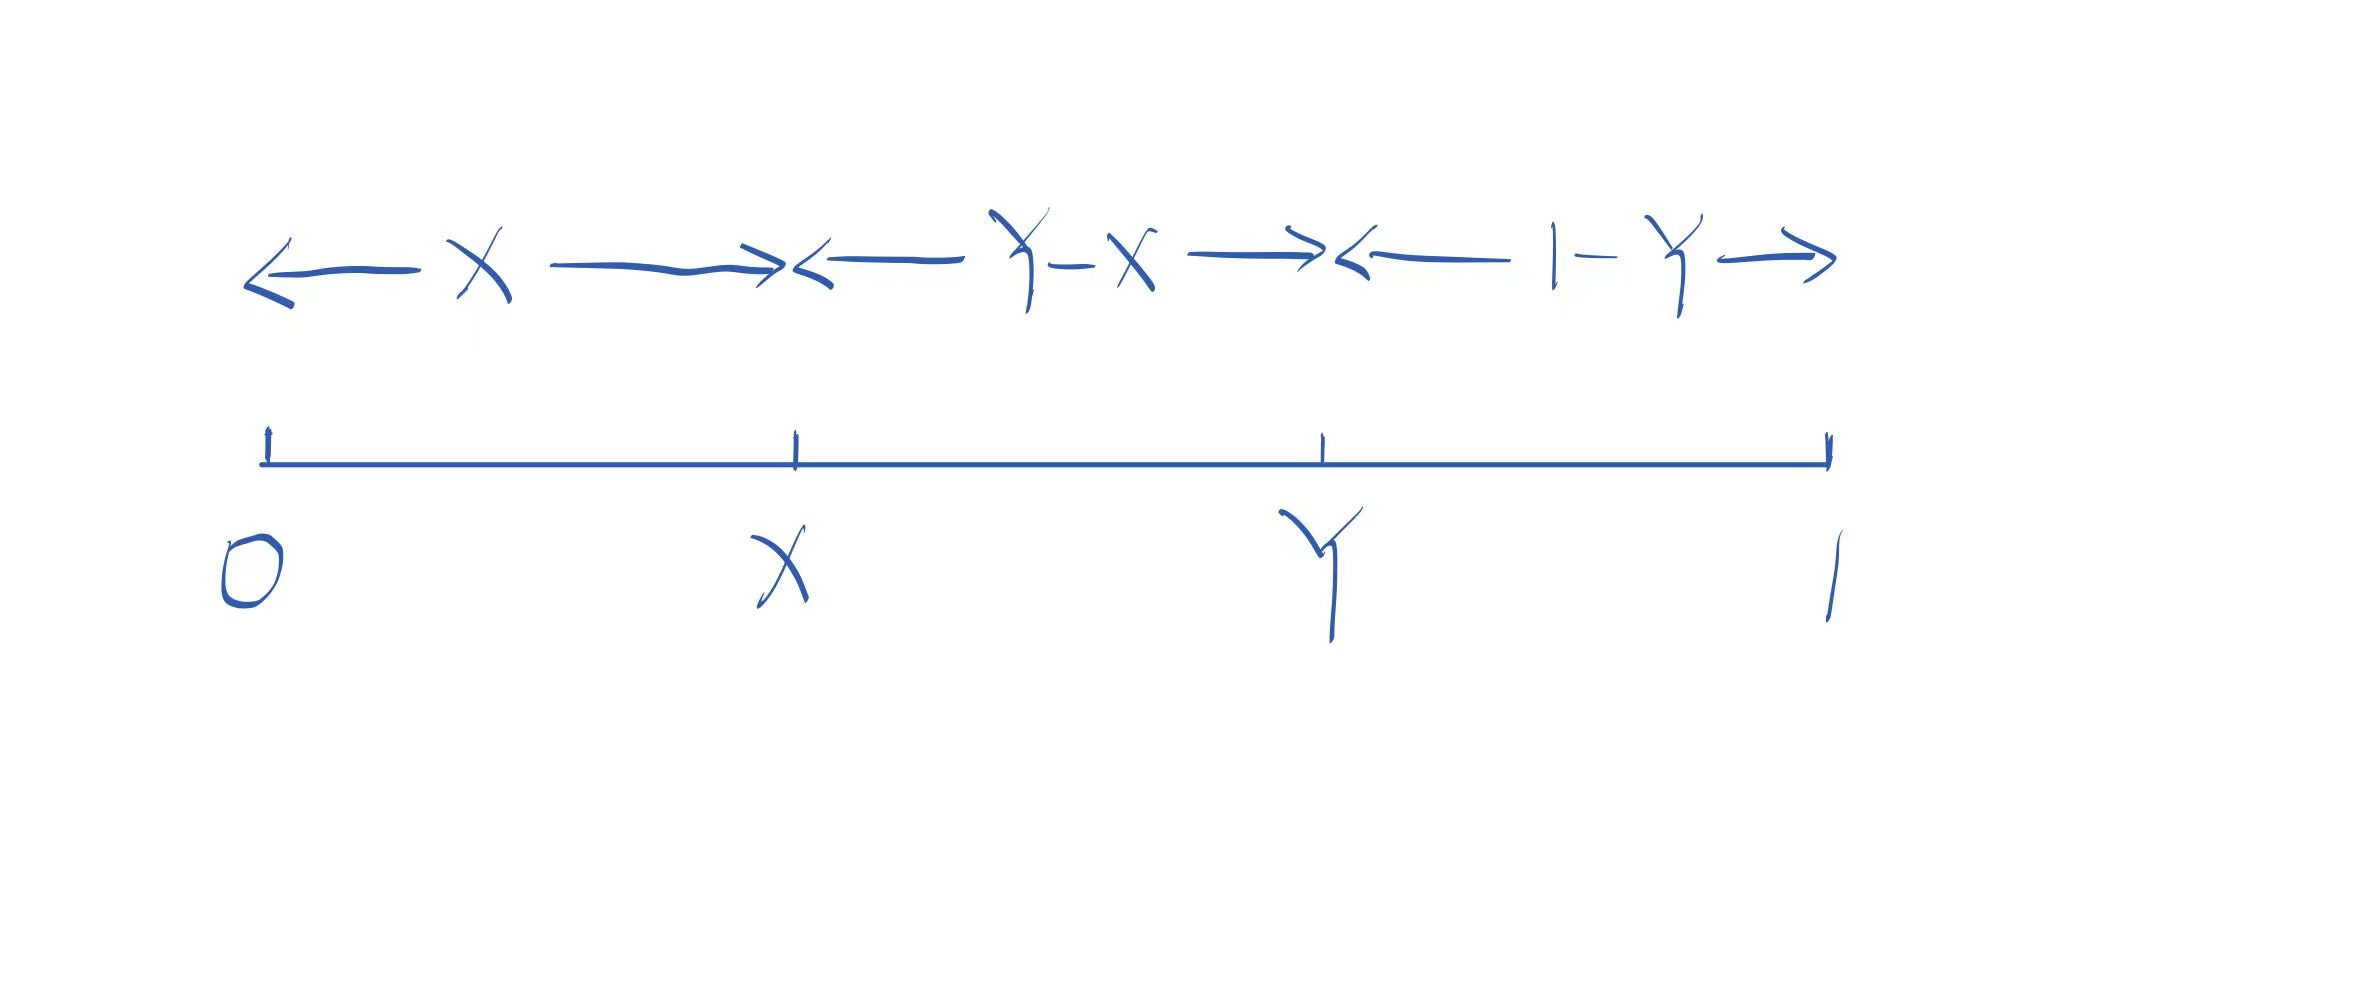
\includegraphics[width=0.7\textwidth]{P1.jpg}
\end{figure}

\[
\begin{cases}
    X + (Y-X) \ge (1-Y) \\
    X + (1-Y) \ge (Y-X) \\
    (Y-X)+(1-Y) \ge X   \\
\end{cases}
\]
\[
\implies
\begin{cases}
    X \le \frac{1}{2}\\
    Y \ge \frac{1}{2}\\
    Y\ge X
\end{cases}
\]


the total eara is the square,the region satisfying the requirements is the shaded area.
\begin{figure}[H]
    \centering
    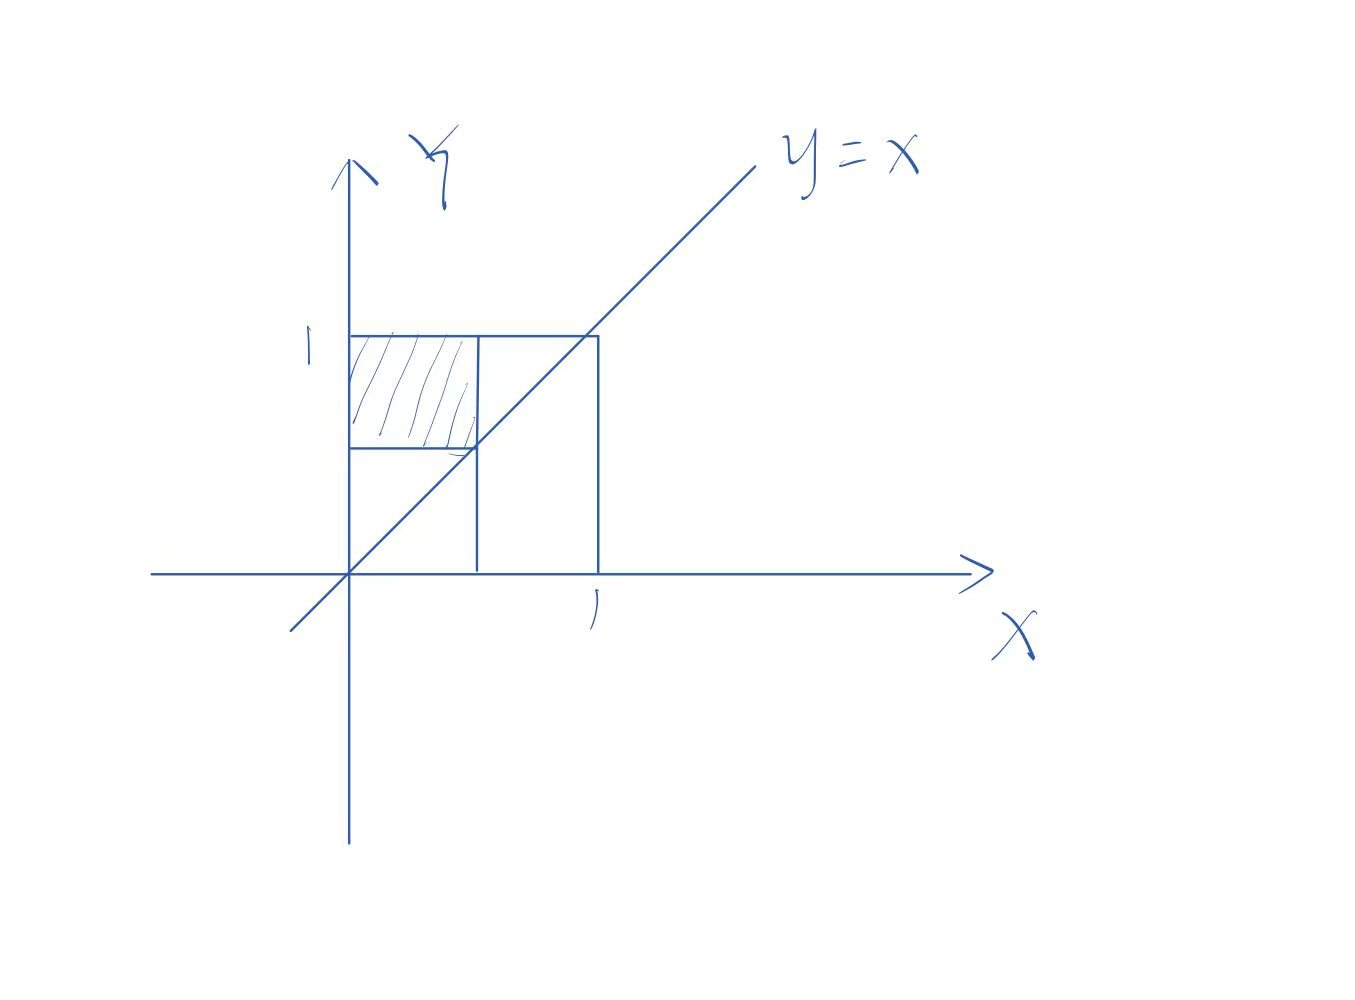
\includegraphics[width=0.7\textwidth]{P2.jpg}
\end{figure}
\[
\therefore
A_{\text{total}}=1*1=1.
\]
\[
A_{\text{shaded}}
=
\frac12\cdot\frac12
=
\frac14.
\]

\[
\implies
P
=
\frac{A_{\text{shaded}}}{A_{\text{total}}}
=
\frac{\frac14}{1}
=
\frac14.
\]



\section*{Problem 4}

Let
\[
\mathbf p=(p_1,p_2,\ldots,p_{365}),
\qquad
\sum_{j=1}^{365}p_j=1.
\]

Recall
\[
e_k(x_1,\ldots,x_n)
=
\sum_{1\le j_1<\cdots<j_k\le n}
x_{j_1}\cdots x_{j_k}.
\]

\subsection*{(a)}
Assume the event that at least one birthday match is A

The probability that all \(k\) birthdays are distinct is B

\[
P(\text{B}\mid \mathbf p)
=
k!
\sum_{1\le j_1<\cdots<j_k\le365}
p_{j_1}\cdots p_{j_k}.
\]

\[
\because
P(\text{all distinct}\mid \mathbf p)
=
k!e_k(p_1,\ldots,p_{365}).
\]

\[
\therefore
P(\text{at least one match}\mid \mathbf p)
=
1-k!e_k(p_1,\ldots,p_{365})
\]

\subsection*{(b)}

For \(k=2\),

\[
P(\text{match})
=
\sum_{j=1}^{365}p_j^2.
\]

If

\[
p_j=\frac1{365},
\]

then

\[
P(\text{match})
=
365\left(\frac1{365}\right)^2
=
\frac1{365}.
\]

In an extreme case,

\[
p_1=1,\qquad
p_2=\cdots=p_{365}=0,
\]

so for \(k\ge2\),

\[
P(\text{at least one match})=1.
\]

Thus, concentrating probability on fewer days increases collisions, while

\[
p_1=p_2=\cdots=p_{365}=\frac1{365}
\]

spreads birthdays most evenly and minimizes the probability of a match.

\subsection*{(c)}

First,

\[
e_k(x_1,\ldots,x_n)
=
x_1x_2e_{k-2}(x_3,\ldots,x_n)
+
(x_1+x_2)e_{k-1}(x_3,\ldots,x_n)
+
e_k(x_3,\ldots,x_n).
\]

Define

\[
r_1=r_2=\frac{p_1+p_2}{2},
\qquad
r_j=p_j,\quad 3\le j\le365.
\]

Then

\[
r_1+r_2=p_1+p_2.
\]

Also, by AM-GM,

\[
\frac{p_1+p_2}{2}\ge\sqrt{p_1p_2},
\]

so

\[
r_1r_2
=
\left(\frac{p_1+p_2}{2}\right)^2
\ge
p_1p_2.
\]

Hence

\[
\begin{aligned}
e_k(\mathbf r)-e_k(\mathbf p)
&=
(r_1r_2-p_1p_2)
e_{k-2}(p_3,\ldots,p_{365})\\
&=
\left[
\left(\frac{p_1+p_2}{2}\right)^2-p_1p_2
\right]
e_{k-2}(p_3,\ldots,p_{365})\\
&=
\frac{(p_1-p_2)^2}{4}
e_{k-2}(p_3,\ldots,p_{365})\\
&\ge0.
\end{aligned}
\]

Therefore,

\[
e_k(\mathbf r)\ge e_k(\mathbf p).
\]

Using part (a),

\[
P(\text{match}\mid\mathbf p)
=
1-k!e_k(\mathbf p),
\]

and

\[
P(\text{match}\mid\mathbf r)
=
1-k!e_k(\mathbf r).
\]

Thus,

\[
P(\text{match}\mid\mathbf p)
\ge
P(\text{match}\mid\mathbf r)
\]

If \(p_1\ne p_2\), then

\[
(p_1-p_2)^2>0,
\]

and hence, when \(e_{k-2}>0\),

\[
P(\text{match}\mid\mathbf p)
>
P(\text{match}\mid\mathbf r).
\]

Thus averaging two unequal probabilities decreases the match probability.

Repeated averaging gives

\[
p_1=p_2=\cdots=p_{365}.
\]

Since

\[
\sum_{j=1}^{365}p_j=1,
\]

we obtain

\[
365p_j=1,
\]

so

\[
p_j=\frac1{365},
\qquad
j=1,\ldots,365
\]

Therefore,

\[
P(\text{at least one birthday match})
\text{ is minimized at }
p_j=\frac1{365}
\]





\section*{Problem 5}

A card collection contains five different types of cards. Each independent draw
produces card type $i$ with probability $p_i$, where
\[
(p_1,p_2,p_3,p_4,p_5)
=
(0.05,0.15,0.20,0.25,0.35).
\]

Let $Q_n$ denote the probability of collecting all five card types after $n$
independent draws.

For each $i\in\{1,\ldots,5\}$, define
\[
E_i
=
\{\text{card type $i$ does not appear in the first $n$ draws}\}.
\]

For any $I\subseteq\{1,\ldots,5\}$, define
\[
E_I=\bigcap_{i\in I}E_i.
\]

\subsection*{(a)}

Collecting all five card types means that none of the events
$E_1,\ldots,E_5$ occurs. Hence
\[
Q_n
=
1-
P\left(\bigcup_{i=1}^{5}E_i\right).
\]

By the inclusion-exclusion principle,
\[
Q_n
=
1
-\sum_{i}P(E_i)
+\sum_{i<j}P(E_i\cap E_j)
-\sum_{i<j<k}P(E_i\cap E_j\cap E_k)
+\cdots.
\]

Based on the question stem
\[
E_I=\bigcap_{i\in I}E_i
\]

For one draw,
\[
P(\text{no type in }I)
=
1-\sum_{i\in I}p_i.
\]

the $n$ draws are independent,
\[
P(E_I)
=
\left(
1-\sum_{i\in I}p_i
\right)^n.
\]


\[
Q_n
=
\sum_{I\subseteq\{1,\ldots,5\}}
(-1)^{|I|}
P(E_I).
\]

\[
\implies
Q_n
=
\sum_{I\subseteq\{1,\ldots,5\}}
(-1)^{|I|}
\left(
1-\sum_{i\in I}p_i
\right)^n
\]

For $I=\varnothing$,
\[
E_{\varnothing}=\Omega,
\qquad
P(E_{\varnothing})=1,
\]
so the term corresponding to $I=\varnothing$ gives the initial $1$ in the
inclusion-exclusion formula.

\subsection*{(b)}

Using
\[
(p_1,p_2,p_3,p_4,p_5)
=
(0.05,0.15,0.20,0.25,0.35),
\]
we compute
\[
Q_n
=
\sum_{I\subseteq\{1,\ldots,5\}}
(-1)^{|I|}
\left(
1-\sum_{i\in I}p_i
\right)^n.
\]

A numerical search gives
\[
Q_{45}=0.8998932711<0.90,
\]
while
\[
Q_{46}=0.9049652386>0.90.
\]

Hence the smallest integer satisfying
\[
Q_n\geq 0.90
\]
is
\[
n=46
\]

The code and terminal output are shown below.

\begin{figure}[h]
    \centering
    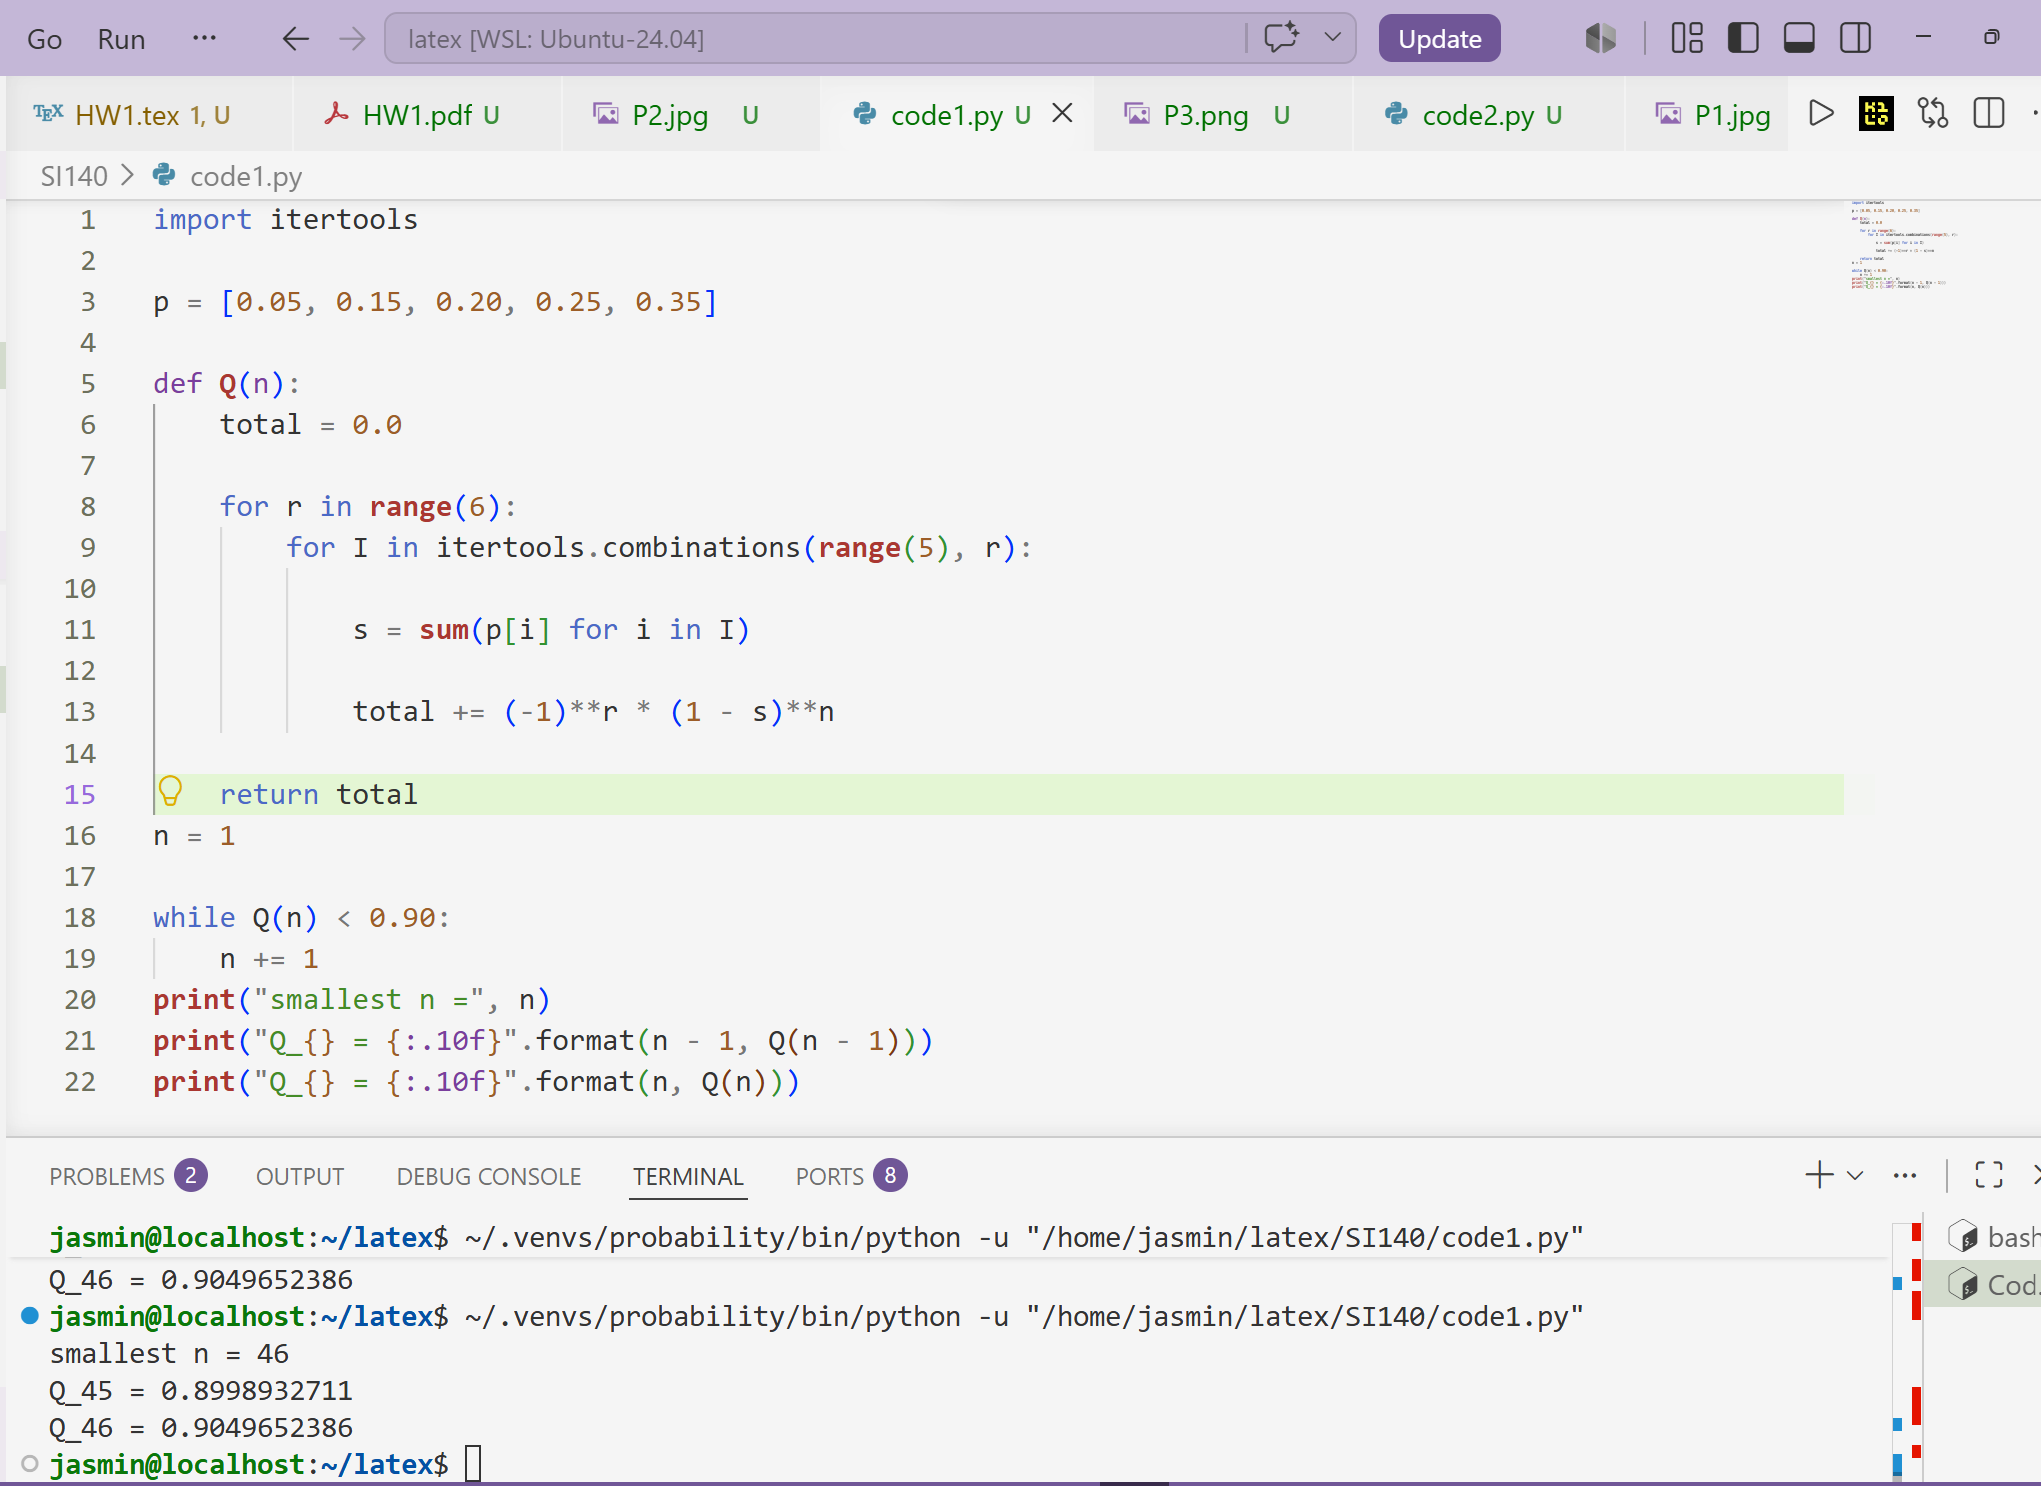
\includegraphics[width=0.9\textwidth]{P3.png}
    \caption{Code and terminal output for part (b).}
\end{figure}

\subsection*{(c)}

\[
p_1=p_2=p_3=p_4=p_5=\frac15.
\]

If $|I|=k$
\[
\implies
\sum_{i\in I}p_i
=
\frac{k}{5}.
\]

\[
\implies
Q_n
=
\sum_{k=0}^{5}
(-1)^k
\binom{5}{k}
\left(
1-\frac{k}{5}
\right)^n.
\]

\[
=
1
-5\left(\frac45\right)^n
+10\left(\frac35\right)^n
-10\left(\frac25\right)^n
+5\left(\frac15\right)^n.
\]

notice that
\[
Q_{17}=0.8891009573<0.90,
\]

\[
Q_{18}=0.9109429198>0.90.
\]

the smallest integer in the uniform case is
\[
n=18
\]

For comparison,
\[
n_{\mathrm{uniform}}=18,
\qquad
n_{\mathrm{unequal}}=46.
\]

The probabilities $Q_n$ for the two cases are plotted below.

\begin{figure}[h]
    \centering
    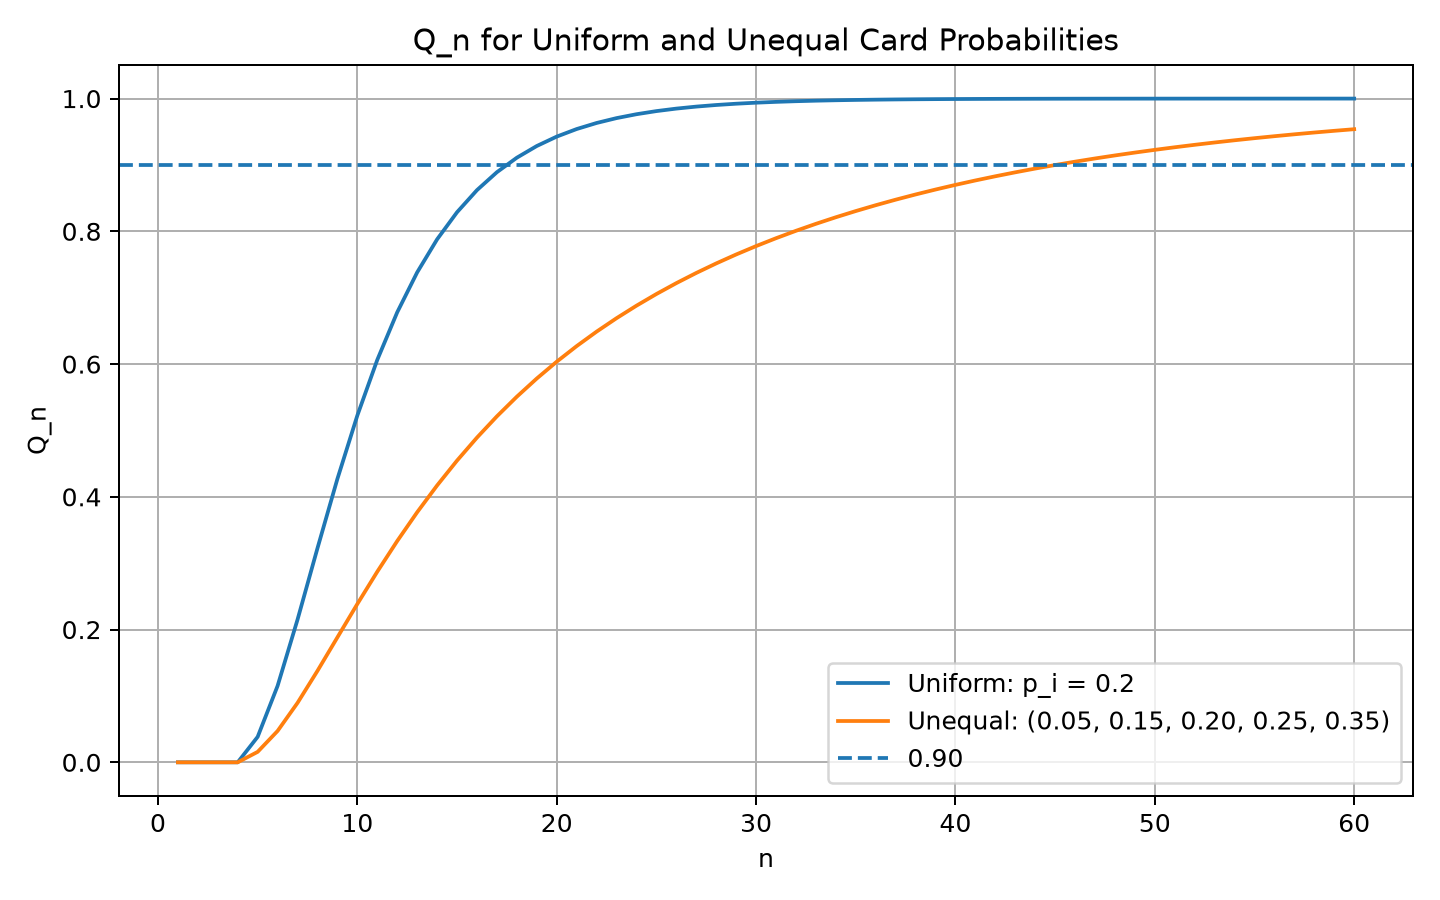
\includegraphics[width=0.85\textwidth]{Qn_equal_vs_unequal.png}
    \caption{$Q_n$ for uniform and unequal card probabilities.}
\end{figure}

From the graph,
\[
Q_n^{\mathrm{uniform}}
>
Q_n^{\mathrm{unequal}}
\]
for the relevant values of $n$.

In the unequal case, the rarest card has probability
\[
p_1=0.05,
\]
so it is much more difficult to collect all five card types. In the uniform
case, every type has probability
\[
p_i=0.20,
\]
so no single card type becomes a bottleneck. Therefore, the probability of
collecting all five types increases much faster in the uniform case.

\end{document}
```
\end{document}

